\documentclass[journal,12pt,onecolumn]{IEEEtran}
\usepackage{cite}
\usepackage{caption}
\usepackage{graphicx}
\usepackage{amsmath,amssymb,amsfonts,amsthm}
\usepackage{algorithmic}
\usepackage{graphicx}
\usepackage{textcomp}
\usepackage{xcolor}
\usepackage{tfrupee}
\usepackage{txfonts}
\usepackage{listings}
\usepackage{enumitem}
\usepackage{mathtools}
\usepackage{gensymb}
\usepackage{comment}
\usepackage[breaklinks=true]{hyperref}
\usepackage{tkz-euclide} 
\usepackage{listings}
\usepackage{gvv}
%\def\inputGnumericTable{}
\usepackage[latin1]{inputenc} 
\usetikzlibrary{arrows.meta, positioning}
\usepackage{xparse}
\usepackage{color}                                            
\usepackage{array}                                            
\usepackage{longtable}                                       
\usepackage{calc}                                             
\usepackage{multirow}
\usepackage{multicol}
\usepackage{hhline}                                           
\usepackage{ifthen}                                           
\usepackage{lscape}
\usepackage{tabularx}
\usepackage{array}
\usepackage{float}
\usepackage{marvosym}
\usepackage{float}
%\newcommand{\define}{\stackrel{\triangle}{=}}
\theoremstyle{remark}
\usepackage{circuitikz}
\captionsetup{justification=centering}
\usepackage{tikz}

\title{Matrices in Geometry 7.4.44}
\author{EE25BTECH11037 - Divyansh}
\begin{document}
\vspace{3cm}
\maketitle
{\let\newpage\relax\maketitle}
\textbf{Question: }
Let C be any circle with centre $\brak{0, \sqrt{2}}$. Prove that at most two rational points can be there on C.  \brak{\text{A rational point is a point both of whose coordinates are rational numbers}}.
\vspace{2mm}


\textbf{Solution:}
\\
The equation of the given circle C can be written as 
\begin{align}
    C: \norm{\vec{x}-\vec{O}}=r
\end{align}
where r is the radius of circle C and $\vec{O}=\myvec{0\\\sqrt{2}}$ is the center of the circle.\\
Let $\vec{P}$ be a rational point on the circle, then
\begin{align}
    \norm{\vec{P} - \vec{O}} = r
\end{align}
Upon squaring both sides,
\begin{align}
    \norm{\vec{P} - \vec{O}}^2 = r^2 \implies \vec{P}^{\top}\vec{P} - 2\vec{P}^{\top}\vec{O} + \vec{O}^{\top}\vec{O} = r^2
\end{align}
Substituting $\vec{P}=\myvec{x \\ y}$ and $\vec{O}=\myvec{0 \\ \sqrt{2}}$
\begin{align}
    \myvec{x & y}\myvec{x \\ y} - 2 \myvec{x&y}\myvec{0 \\ \sqrt{2}} + \myvec{0 & \sqrt{2}}\myvec{0 \\ \sqrt{2}} = r^2\\
    \implies x^2 + y^2 - 2\sqrt{2}y + 2=r^2
\end{align}
Rearranging the terms,
\begin{align}
    x^2 + y^2 -r^2 + 2=2\sqrt{2}y\\
    \vec{P} \in R^2 \implies x, y \in R \implies \text{LHS is rational} \implies \text{RHS should be rational} \\
    \implies y=0 \\
    \therefore x^2 = r^2 -2 \implies x = \pm \sqrt{r^2 - 2}: r>\sqrt{2}
\end{align}

We get the points 
\begin{align}
    \vec{P}=\myvec{\sqrt{r^2 - 2}\\0} \text{ OR } \vec{P} = \myvec{-\sqrt{r^2 - 2}\\0} : r^2 - 2 \text{ is a perfect square} 
\end{align}
This proves that at most two rational points can be present in C.\\
Let us try to show this using a graph with $r=\sqrt{6}$.
\begin{figure}[H]
    \centering
    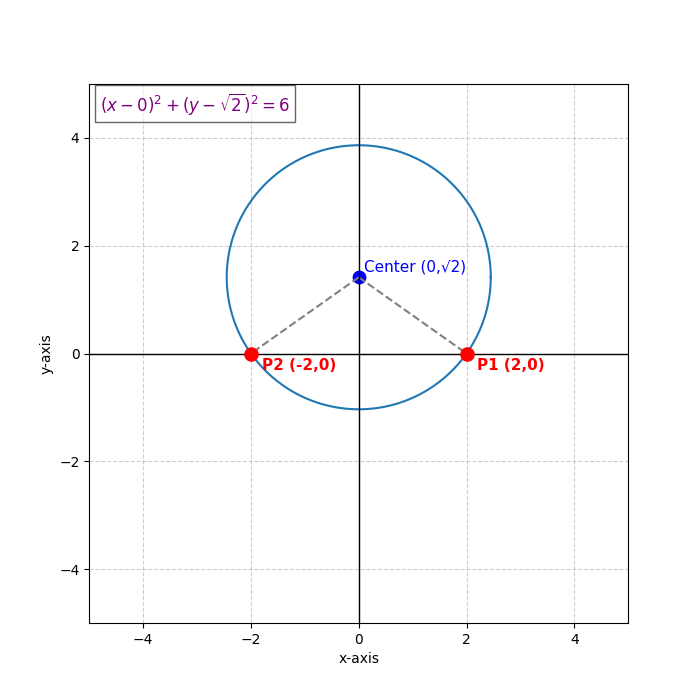
\includegraphics[width=1\columnwidth]{figs/1.png}
    \caption{Graph for 7.4.44 with $r= \sqrt{6}$}
    \label{fig:placeholder}
\end{figure}
\end{document}
